% ============================================================================
% CSCE 775: Deep Reinforcement Learning - Homework 1 SOLUTIONS
% ============================================================================

\documentclass[12pt]{article}

% ============================================================================
% PACKAGE IMPORTS
% ============================================================================
\usepackage{amsmath}
\usepackage{graphicx}
\usepackage{amssymb}
\usepackage{tikz}
\usepackage[margin=1in]{geometry}
\usepackage{setspace}
\usepackage{xcolor}
\usepackage{enumitem}
\usepackage{tcolorbox}
\usepackage{fancyhdr}
\usepackage{booktabs}
\usepackage{array}
\usepackage{colortbl}
\usepackage{float}
\usepackage{bm}
\usepackage{pgfplots}
\pgfplotsset{compat=1.18}

% ============================================================================
% HEADER AND FOOTER SETUP
% ============================================================================
\pagestyle{fancy}
\setlength{\headheight}{14.5pt}
\fancyhf{}

\fancyhead[L]{Page \thepage}
\fancyhead[C]{CSCE 775}
\fancyhead[R]{JC Vaught}

\renewcommand{\headrulewidth}{0pt}

% ============================================================================
% TIKZ LIBRARIES
% ============================================================================
\usetikzlibrary{shapes.geometric, arrows.meta, positioning, automata, calc, decorations.markings, patterns}

% --- USC Brand Colors ---
\definecolor{USC_Garnet}{HTML}{73000A}
\definecolor{USC_Sandstorm}{HTML}{FFF2E3}
\definecolor{USC_Black90}{HTML}{363636}
\definecolor{USC_Black70}{HTML}{5C5C5C}
\definecolor{USC_Black50}{HTML}{A2A2A2}
\definecolor{USC_Black10}{HTML}{ECECEC}
\definecolor{USC_Honeycomb}{HTML}{A49137}
\definecolor{USC_Horseshoe}{HTML}{65780B}
\definecolor{USC_Atlantic}{HTML}{466A9F}
\definecolor{USC_Congaree}{HTML}{1F414D}
\definecolor{USC_Rose}{HTML}{CC2E40}

% ============================================================================
% CUSTOM COLORED BOXES
% ============================================================================
\newtcolorbox{stepbox}[1][Step]{
  colback=white,
  colframe=USC_Garnet,
  fonttitle=\bfseries,
  title=#1,
  sharp corners,
  colbacktitle=USC_Garnet,
  coltitle=white,
}

\newtcolorbox{resultsbox}{
  colback=white,
  colframe=USC_Horseshoe,
  fonttitle=\bfseries,
  title=Results,
  sharp corners,
  colbacktitle=USC_Horseshoe,
  coltitle=white,
}

\newtcolorbox{problembox}[1][Problem]{
  colback=USC_Black10,
  colframe=USC_Black90,
  fonttitle=\bfseries,
  title=#1,
  sharp corners,
  colbacktitle=USC_Black90,
  coltitle=white,
}

% ============================================================================
% CUSTOM QUESTION AND PART COMMANDS
% ============================================================================
\newcommand{\question}[1]{%
  \clearpage
  \vspace{0.5cm}
  {\noindent\normalsize \textbf{#1}}
  \vspace{0.2cm}
  \hrule
  \vspace{0.1cm}
  \hrule
  \vspace{0.3cm}
}

\newcommand{\questionpart}[1]{%
  \vspace{0.8cm}
  {\noindent\normalsize \textbf{#1}}
  \vspace{0.2cm}
  \hrule
  \vspace{0.1cm}
  \hrule
  \vspace{0.3cm}
}

% ============================================================================
% DOCUMENT INFORMATION
% ============================================================================

\title{CSCE 775: Deep Reinforcement Learning \\ Homework \#1 --- Solutions}
\author{Instructor: Dr.\ Forest Agostinelli \\ University of South Carolina \\ \textit{Solutions by: J.C.\ Vaught}}
\date{Spring 2026}

% ============================================================================
% BEGIN DOCUMENT
% ============================================================================

\begin{document}

\maketitle
\setlength{\parindent}{0pt}

\setlist[enumerate,1]{label=\arabic*.}
\setlist[enumerate,2]{label=(\alph*)}

% ============================================================================
% TABLE OF CONTENTS
% ============================================================================

\begin{center}
\begin{tcolorbox}[colback=white, colframe=gray!50!black, colbacktitle=gray!20!white,
                  coltitle=black, sharp corners, boxrule=1pt,
                  title=\Large\bfseries Table of Contents]
\begin{tabular}{p{0.82\textwidth}r}
\textbf{Problem 1: MRP State Values} \dotfill & \textbf{\pageref{prob:mrp}} \\[0.3em]
\textbf{Problem 2: MRP Discount Factor Analysis} \dotfill & \textbf{\pageref{prob:discount}} \\[0.3em]
\textbf{Problem 3: Value Iteration by Hand} \dotfill & \textbf{\pageref{prob:vi}} \\[0.3em]
\textbf{Problem 4: Grid World Policy} \dotfill & \textbf{\pageref{prob:grid}} \\[0.3em]
\textbf{Problem 5: Q-Learning Episode Trace} \dotfill & \textbf{\pageref{prob:qlearn}} \\[0.3em]
\textbf{Problem 6: Exploration vs.\ Exploitation} \dotfill & \textbf{\pageref{prob:explore}} \\
\end{tabular}
\vspace{0.2cm}
\end{tcolorbox}
\end{center}

% ============================================================================
% PROBLEM 1: MRP State Values
% ============================================================================

\question{Problem 1: MRP State Values}\label{prob:mrp}

Consider the following Markov Reward Process with three states $\mathcal{S} = \{S_1, S_2, S_3\}$.

\begin{center}
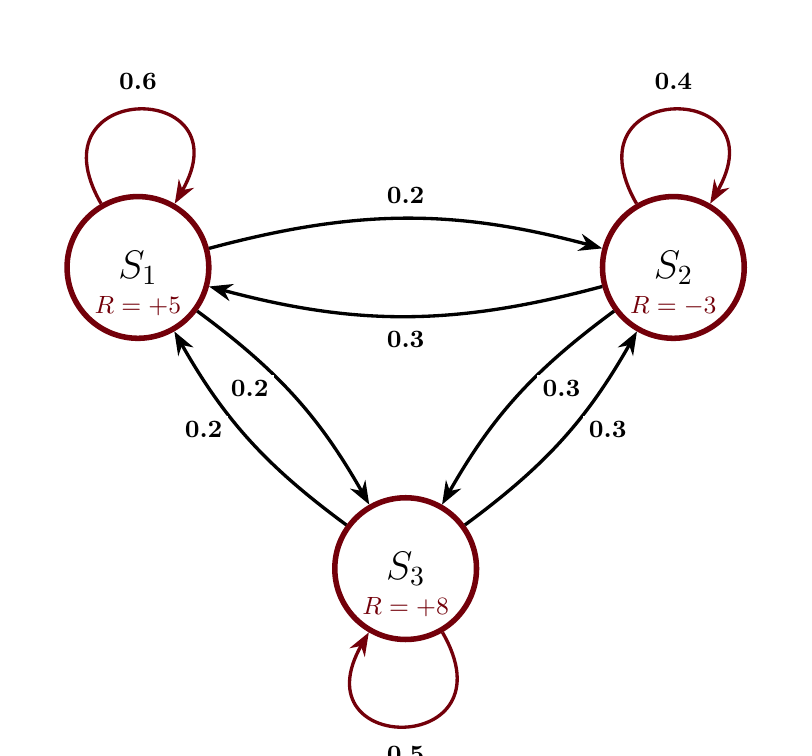
\begin{tikzpicture}[
    >=Stealth,
    scale=0.85,
    every state/.style={
        fill=white,
        draw=USC_Garnet,
        line width=2pt,
        text=black,
        minimum size=1.8cm,
        font=\bfseries\Large
    },
    every edge/.style={
        draw=black,
        line width=1.2pt,
        ->,
        >=Stealth
    },
    prob/.style={
        font=\bfseries\small,
        text=black,
        fill=white,
        inner sep=2pt
    },
    statelabel/.style={
        font=\small\bfseries,
        text=USC_Garnet
    }
]

\node[state] (S1) at (0, 0) {$S_1$};
\node[statelabel, below=1pt of S1.center, yshift=-6pt] {$R=+5$};

\node[state] (S2) at (8, 0) {$S_2$};
\node[statelabel, below=1pt of S2.center, yshift=-6pt] {$R=-3$};

\node[state] (S3) at (4, -4.5) {$S_3$};
\node[statelabel, below=1pt of S3.center, yshift=-6pt] {$R=+8$};

\path (S1) edge[loop above, looseness=5, out=120, in=60, draw=USC_Garnet] node[prob, above=5pt] {0.6} (S1);
\path (S2) edge[loop above, looseness=5, out=120, in=60, draw=USC_Garnet] node[prob, above=5pt] {0.4} (S2);
\path (S3) edge[loop below, looseness=5, out=-60, in=-120, draw=USC_Garnet] node[prob, below=5pt] {0.5} (S3);

\path (S1) edge[bend left=15] node[prob, above=3pt] {0.2} (S2);
\path (S2) edge[bend left=15] node[prob, below=3pt] {0.3} (S1);

\path (S1) edge[bend left=12] node[prob, left=4pt, pos=0.45] {0.2} (S3);
\path (S3) edge[bend left=12] node[prob, left=4pt, pos=0.55] {0.2} (S1);

\path (S2) edge[bend right=12] node[prob, right=4pt, pos=0.45] {0.3} (S3);
\path (S3) edge[bend right=12] node[prob, right=4pt, pos=0.55] {0.3} (S2);

\end{tikzpicture}
\end{center}

The transition matrix and reward vector are:
\[
\mathcal{P} = \begin{pmatrix}
0.6 & 0.2 & 0.2 \\
0.3 & 0.4 & 0.3 \\
0.2 & 0.3 & 0.5
\end{pmatrix}, \qquad
\mathbf{R} = \begin{pmatrix} +5 \\ -3 \\ +8 \end{pmatrix}
\]

\begin{enumerate}[label=(\alph*)]
\item Write the Bellman equation for this MRP in matrix form for a general discount factor $\gamma$. That is, express $\mathbf{V}$ as a function of $\mathbf{R}$, $\gamma$, and $\mathcal{P}$.

\begin{stepbox}[Solution 1(a)]
The Bellman equation for an MRP is $\mathbf{V} = \mathbf{R} + \gamma \mathcal{P}\mathbf{V}$. Rearranging:
\[
(\mathbf{I} - \gamma \mathcal{P})\mathbf{V} = \mathbf{R}
\]
\end{stepbox}
\begin{resultsbox}
\[
\boxed{\mathbf{V} = (\mathbf{I} - \gamma \mathcal{P})^{-1}\mathbf{R}}
\]
\end{resultsbox}

\item Form the matrix $(\mathbf{I} - \gamma \mathcal{P})$ explicitly for $\gamma = 0.8$. Show all entries.

\begin{stepbox}[Solution 1(b)]
\[
\mathbf{I} - 0.8\mathcal{P} = \begin{pmatrix} 1 & 0 & 0 \\ 0 & 1 & 0 \\ 0 & 0 & 1 \end{pmatrix} - 0.8\begin{pmatrix} 0.6 & 0.2 & 0.2 \\ 0.3 & 0.4 & 0.3 \\ 0.2 & 0.3 & 0.5 \end{pmatrix}
\]
\end{stepbox}
\begin{resultsbox}
\[
\boxed{\mathbf{I} - 0.8\mathcal{P} = \begin{pmatrix} 0.52 & -0.16 & -0.16 \\ -0.24 & 0.68 & -0.24 \\ -0.16 & -0.24 & 0.60 \end{pmatrix}}
\]
\end{resultsbox}

\item Solve the $3 \times 3$ linear system $(\mathbf{I} - \gamma \mathcal{P})\mathbf{V} = \mathbf{R}$ for $\gamma = 0.8$ to find $V(S_1)$, $V(S_2)$, and $V(S_3)$. Show your work.

\begin{stepbox}[Solution 1(c) --- Cramer's Rule]
We solve:
\[
\begin{pmatrix} 0.52 & -0.16 & -0.16 \\ -0.24 & 0.68 & -0.24 \\ -0.16 & -0.24 & 0.60 \end{pmatrix} \begin{pmatrix} V_1 \\ V_2 \\ V_3 \end{pmatrix} = \begin{pmatrix} 5 \\ -3 \\ 8 \end{pmatrix}
\]

\textbf{Determinant of $A = \mathbf{I} - 0.8\mathcal{P}$:}
\begin{align*}
\det(A) &= 0.52(0.68 \cdot 0.60 - (-0.24)(-0.24)) \\
        &\quad - (-0.16)((-0.24)(0.60) - (-0.24)(-0.16)) \\
        &\quad + (-0.16)((-0.24)(-0.24) - (0.68)(-0.16)) \\
        &= 0.52(0.4080 - 0.0576) + 0.16(-0.1440 - 0.0384) - 0.16(0.0576 + 0.1088) \\
        &= 0.52(0.3504) + 0.16(-0.1824) - 0.16(0.1664) \\
        &= 0.18221 - 0.02918 - 0.02662 = 0.12640
\end{align*}

\textbf{For $V_1$} (replace column 1 with $\mathbf{R}$):
\begin{align*}
\det(A_1) &= 5(0.408 - 0.0576) + 0.16(-1.8 + 1.92) - 0.16(0.72 - 5.44) \\
          &= 5(0.3504) + 0.16(0.12) - 0.16(-4.72) \\
          &= 1.7520 + 0.0192 + 0.7552 = 2.5264
\end{align*}

\textbf{For $V_2$} (replace column 2 with $\mathbf{R}$):
\begin{align*}
\det(A_2) &= 0.52(-1.8 + 1.92) - 5(-0.144 - 0.0384) - 0.16(-1.92 - 0.48) \\
          &= 0.52(0.12) - 5(-0.1824) - 0.16(-2.4) \\
          &= 0.0624 + 0.9120 + 0.3840 = 1.3584
\end{align*}

\textbf{For $V_3$} (replace column 3 with $\mathbf{R}$):
\begin{align*}
\det(A_3) &= 0.52(5.44 - 0.72) + 0.16(-1.92 - 0.48) + 5(0.0576 + 0.1088) \\
          &= 0.52(4.72) + 0.16(-2.4) + 5(0.1664) \\
          &= 2.4544 - 0.3840 + 0.8320 = 2.9024
\end{align*}
\end{stepbox}

\begin{resultsbox}
\[
\boxed{V(S_1) = \frac{2.5264}{0.1264} \approx 19.99}, \qquad
\boxed{V(S_2) = \frac{1.3584}{0.1264} \approx 10.75}, \qquad
\boxed{V(S_3) = \frac{2.9024}{0.1264} \approx 22.96}
\]
\end{resultsbox}

\end{enumerate}

% ============================================================================
% PROBLEM 2: Discount Factor Analysis
% ============================================================================

\question{Problem 2: MRP Discount Factor Analysis}\label{prob:discount}

Use the same MRP from Problem~1.

\begin{enumerate}[label=(\alph*)]
\item Compute $V(S_1)$, $V(S_2)$, and $V(S_3)$ for $\gamma = 0$. Briefly explain why the answer is immediate.

\begin{stepbox}[Solution 2(a)]
When $\gamma = 0$, the Bellman equation becomes $\mathbf{V} = \mathbf{R} + 0 \cdot \mathcal{P}\mathbf{V} = \mathbf{R}$. The agent is completely myopic---it only values the immediate reward with no consideration of future states.
\end{stepbox}
\begin{resultsbox}
\[
\boxed{V(S_1) = 5, \qquad V(S_2) = -3, \qquad V(S_3) = 8}
\]
\end{resultsbox}

\item Compute $V(S_1)$, $V(S_2)$, and $V(S_3)$ for $\gamma = 0.5$.

\begin{stepbox}[Solution 2(b)]
Form $\mathbf{I} - 0.5\mathcal{P}$:
\[
\mathbf{I} - 0.5\mathcal{P} = \begin{pmatrix} 0.70 & -0.10 & -0.10 \\ -0.15 & 0.80 & -0.15 \\ -0.10 & -0.15 & 0.75 \end{pmatrix}
\]

Using Cramer's rule (same procedure as Problem~1(c)):
\[
\det(\mathbf{I} - 0.5\mathcal{P}) = 0.38125
\]
\[
\det(A_1) = 3.3775, \quad \det(A_2) = 0.0525, \quad \det(A_3) = 4.5275
\]
\end{stepbox}
\begin{resultsbox}
\[
\boxed{V(S_1) \approx 8.86}, \qquad \boxed{V(S_2) \approx 0.14}, \qquad \boxed{V(S_3) \approx 11.88}
\]
\end{resultsbox}

\item For approximately what value of $\gamma$ does $V(S_2)$ cross from negative to positive? Set $V(S_2) = 0$ in the Bellman equation and solve.

\begin{stepbox}[Solution 2(c)]
Set $V(S_2) = 0$ in the Bellman equation. From the second row:
\[
V(S_2) = -3 + \gamma[0.3V(S_1) + 0.4 \cdot 0 + 0.3V(S_3)] = 0 \implies V(S_1) + V(S_3) = \frac{10}{\gamma}
\]
From the first and third rows (with $V(S_2)=0$):
\[
V(S_1)(1 - 0.6\gamma) = 5 + 0.2\gamma V(S_3), \qquad V(S_3)(1 - 0.5\gamma) = 8 + 0.2\gamma V(S_1)
\]
Substituting $V(S_1) = 10/\gamma - V(S_3)$ into the third equation yields $V(S_3) = 10/(1 - 0.3\gamma)$. Substituting both into the first equation and simplifying:
\[
7.3\gamma^2 - 24\gamma + 10 = 0
\]
\[
\gamma = \frac{24 - \sqrt{576 - 292}}{14.6} = \frac{24 - \sqrt{284}}{14.6} = \frac{24 - 16.852}{14.6}
\]
\end{stepbox}
\begin{resultsbox}
\[
\boxed{\gamma \approx 0.49}
\]
\end{resultsbox}

\item On the axes below, sketch the curves $V(S_1)$, $V(S_2)$, and $V(S_3)$ as functions of $\gamma \in [0, 1)$. Label each curve and mark the zero-crossing from part~(c).

\begin{center}
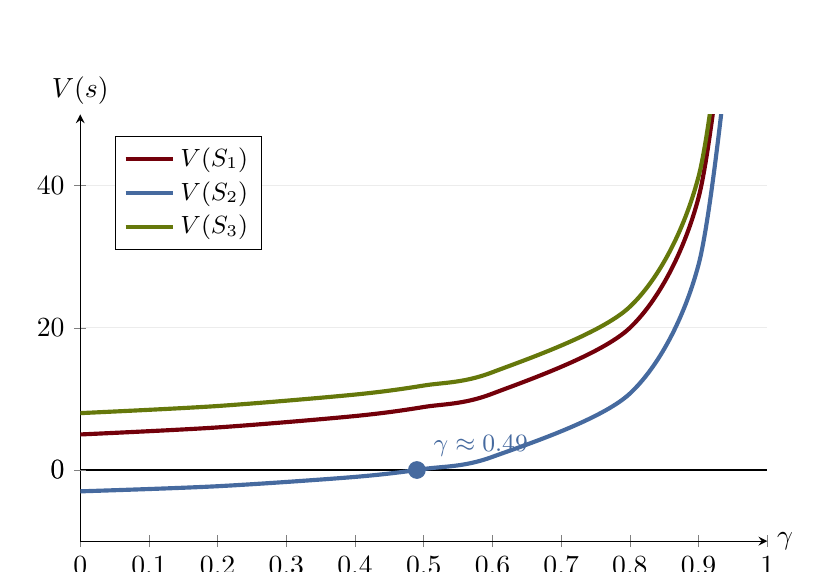
\begin{tikzpicture}
\begin{axis}[
    width=0.85\textwidth,
    height=7cm,
    xlabel={$\gamma$},
    ylabel={$V(s)$},
    xmin=0, xmax=1,
    ymin=-10, ymax=50,
    ymajorgrids=true,
    grid style={USC_Black10},
    axis lines=left,
    every axis x label/.style={at={(ticklabel* cs:1.0)}, anchor=west},
    every axis y label/.style={at={(ticklabel* cs:1.0)}, anchor=south},
    extra y ticks={0},
    extra y tick style={grid=major, grid style={black, line width=0.5pt}},
    legend style={at={(0.05,0.95)}, anchor=north west, font=\small},
]
% V(S1)
\addplot[color=USC_Garnet, line width=1.5pt, mark=none, smooth]
    coordinates {
        (0, 5.00) (0.2, 5.99) (0.4, 7.59) (0.5, 8.86)
        (0.6, 10.74) (0.8, 19.99) (0.9, 38.33) (0.95, 74.91)
    };
\addlegendentry{$V(S_1)$}

% V(S2)
\addplot[color=USC_Atlantic, line width=1.5pt, mark=none, smooth]
    coordinates {
        (0, -3.00) (0.2, -2.28) (0.4, -0.97) (0.5, 0.14)
        (0.6, 1.85) (0.8, 10.75) (0.9, 28.89) (0.95, 65.37)
    };
\addlegendentry{$V(S_2)$}

% V(S3)
\addplot[color=USC_Horseshoe, line width=1.5pt, mark=none, smooth]
    coordinates {
        (0, 8.00) (0.2, 9.00) (0.4, 10.61) (0.5, 11.88)
        (0.6, 13.75) (0.8, 22.96) (0.9, 41.27) (0.95, 77.83)
    };
\addlegendentry{$V(S_3)$}

% Zero-crossing marker
\addplot[only marks, mark=*, mark size=3pt, color=USC_Atlantic]
    coordinates {(0.49, 0)};
\node[anchor=south west, font=\small\bfseries, text=USC_Atlantic] at (axis cs:0.50, 0.5) {$\gamma \approx 0.49$};

\end{axis}
\end{tikzpicture}
\end{center}
\end{enumerate}

% ============================================================================
% PROBLEM 3: Value Iteration by Hand
% ============================================================================

\question{Problem 3: Value Iteration by Hand}\label{prob:vi}

Consider the following MDP with states $\{X, Y\}$ and a terminal state $Z_T$, discount factor $\gamma = 0.9$. Each non-terminal state has two actions: $a_1$ and $a_2$. All transitions are deterministic.

\begin{center}
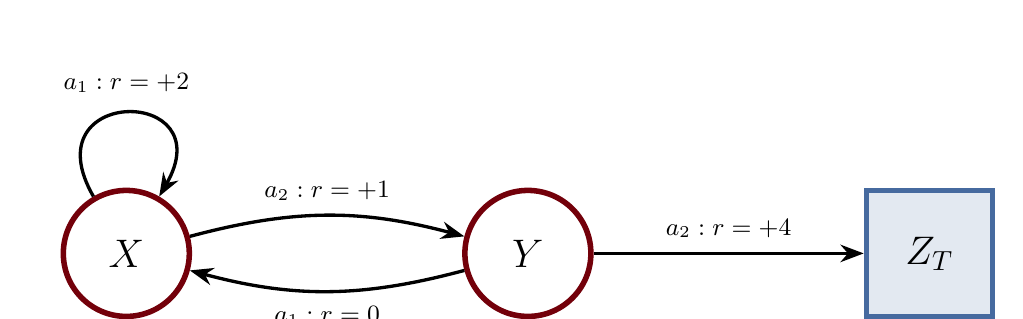
\begin{tikzpicture}[
    >=Stealth,
    scale=0.85,
    every state/.style={
        fill=white,
        draw=USC_Garnet,
        line width=2pt,
        text=black,
        minimum size=1.6cm,
        font=\bfseries\Large
    },
    every edge/.style={draw=black, line width=1.2pt, ->, >=Stealth},
    prob/.style={font=\small\bfseries, fill=white, inner sep=2pt},
    term/.style={
        fill=USC_Atlantic!15,
        draw=USC_Atlantic,
        line width=2pt,
        text=black,
        minimum size=1.6cm,
        font=\bfseries\Large
    }
]

\node[state] (X) at (0, 0) {$X$};
\node[state] (Y) at (6, 0) {$Y$};
\node[term] (Z) at (12, 0) {$Z_T$};

\path (X) edge[loop above, looseness=5, out=120, in=60] node[prob, above=5pt] {$a_1: r=+2$} (X);
\path (X) edge[bend left=15] node[prob, above=3pt] {$a_2: r=+1$} (Y);

\path (Y) edge[bend left=15] node[prob, below=3pt] {$a_1: r=0$} (X);
\path (Y) edge node[prob, above=3pt] {$a_2: r=+4$} (Z);

\end{tikzpicture}
\end{center}

\textbf{Transition and reward summary:}
\begin{center}
\begin{tabular}{cccc}
\toprule
\textbf{State} & \textbf{Action} & \textbf{Next State} & \textbf{Reward} \\
\midrule
$X$ & $a_1$ & $X$ & $+2$ \\
$X$ & $a_2$ & $Y$ & $+1$ \\
$Y$ & $a_1$ & $X$ & $0$ \\
$Y$ & $a_2$ & $Z_T$ & $+4$ \\
\bottomrule
\end{tabular}
\end{center}

\begin{enumerate}[label=(\alph*)]
\item Initialize $V_0(X) = V_0(Y) = 0$. Perform \textbf{3 iterations} of value iteration. Fill in the table below. Show computation for each cell.

\begin{stepbox}[Solution 3(a)]
Value iteration update: $V_{k+1}(s) = \max_a \big[R(s,a) + \gamma V_k(s')\big]$

\textbf{Iteration 1} ($V_0(X) = V_0(Y) = 0$):
\begin{align*}
Q(X, a_1) &= 2 + 0.9 \cdot V_0(X) = 2 + 0 = 2 \\
Q(X, a_2) &= 1 + 0.9 \cdot V_0(Y) = 1 + 0 = 1 \\
V_1(X) &= \max(2, 1) = 2, \quad \pi_1(X) = a_1
\end{align*}
\begin{align*}
Q(Y, a_1) &= 0 + 0.9 \cdot V_0(X) = 0 \\
Q(Y, a_2) &= 4 + 0.9 \cdot 0 = 4 \\
V_1(Y) &= \max(0, 4) = 4, \quad \pi_1(Y) = a_2
\end{align*}

\textbf{Iteration 2} ($V_1(X) = 2,\; V_1(Y) = 4$):
\begin{align*}
Q(X, a_1) &= 2 + 0.9(2) = 3.8 \\
Q(X, a_2) &= 1 + 0.9(4) = 4.6 \\
V_2(X) &= 4.6, \quad \pi_2(X) = a_2
\end{align*}
\begin{align*}
Q(Y, a_1) &= 0 + 0.9(2) = 1.8 \\
Q(Y, a_2) &= 4 + 0.9(0) = 4 \\
V_2(Y) &= 4, \quad \pi_2(Y) = a_2
\end{align*}

\textbf{Iteration 3} ($V_2(X) = 4.6,\; V_2(Y) = 4$):
\begin{align*}
Q(X, a_1) &= 2 + 0.9(4.6) = 6.14 \\
Q(X, a_2) &= 1 + 0.9(4) = 4.6 \\
V_3(X) &= 6.14, \quad \pi_3(X) = a_1
\end{align*}
\begin{align*}
Q(Y, a_1) &= 0 + 0.9(4.6) = 4.14 \\
Q(Y, a_2) &= 4 + 0 = 4 \\
V_3(Y) &= 4.14, \quad \pi_3(Y) = a_1
\end{align*}
\end{stepbox}

\begin{resultsbox}
\begin{center}
\begin{tabular}{ccccc}
\toprule
\textbf{Iter $k$} & $V_k(X)$ & $\pi_k(X)$ & $V_k(Y)$ & $\pi_k(Y)$ \\
\midrule
0 & 0 & --- & 0 & --- \\[0.5em]
1 & 2.00 & $a_1$ & 4.00 & $a_2$ \\[0.5em]
2 & 4.60 & $a_2$ & 4.00 & $a_2$ \\[0.5em]
3 & 6.14 & $a_1$ & 4.14 & $a_1$ \\
\bottomrule
\end{tabular}
\end{center}
\end{resultsbox}

\item After convergence, what is the optimal policy $\pi^*$? State $\pi^*(X)$ and $\pi^*(Y)$ and justify briefly.

\begin{stepbox}[Solution 3(b)]
At convergence, the optimal policy is $\pi^*(X) = a_1$ and $\pi^*(Y) = a_1$. From state $X$, taking $a_1$ yields reward $+2$ and stays in $X$, accumulating $2/(1-0.9) = 20$ in total discounted reward. Taking $a_2$ would move to $Y$ with reward $+1$, which is suboptimal. From state $Y$, taking $a_1$ transitions to $X$ (reward 0) and then the agent collects the stream of $+2$'s; this is worth $0.9 \cdot 20 = 18$, which exceeds $a_2$'s value of $4$.
\end{stepbox}
\begin{resultsbox}
\[
\boxed{\pi^*(X) = a_1, \qquad \pi^*(Y) = a_1}
\]
\end{resultsbox}

\item Compute the exact optimal values $V^*(X)$ and $V^*(Y)$ by solving the Bellman optimality equations simultaneously.

\begin{stepbox}[Solution 3(c)]
Assuming $\pi^*(X) = a_1$ and $\pi^*(Y) = a_1$ (verified by checking all Q-values):
\begin{align*}
V^*(X) &= 2 + 0.9\,V^*(X) \implies V^*(X)(1 - 0.9) = 2 \implies V^*(X) = 20 \\
V^*(Y) &= 0 + 0.9\,V^*(X) = 0.9 \cdot 20 = 18
\end{align*}

\textbf{Verification:} $Q(X, a_2) = 1 + 0.9(18) = 17.2 < 20 = Q(X, a_1)$ \checkmark \\
$Q(Y, a_2) = 4 + 0 = 4 < 18 = Q(Y, a_1)$ \checkmark
\end{stepbox}
\begin{resultsbox}
\[
\boxed{V^*(X) = 20, \qquad V^*(Y) = 18}
\]
\end{resultsbox}

\end{enumerate}

% ============================================================================
% PROBLEM 4: Grid World Policy
% ============================================================================

\question{Problem 4: Grid World Policy}\label{prob:grid}

Consider the $3 \times 3$ grid MDP below. The agent can move \textbf{Up, Down, Left, Right}. Moves that would leave the grid keep the agent in place. All transitions are deterministic. Discount factor $\gamma = 1$.

\begin{center}
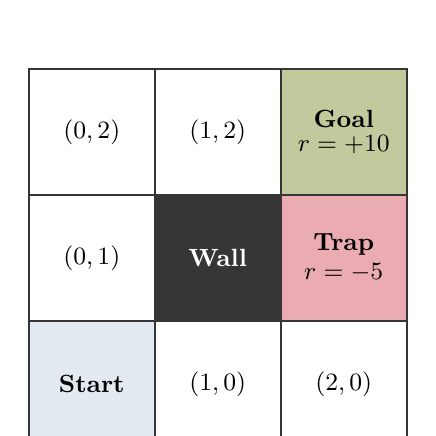
\begin{tikzpicture}[
    cell/.style={minimum size=1.6cm, draw=USC_Black90, line width=0.8pt, font=\small, anchor=center}
]

\node[cell, fill=white] at (0, 3.2) {$(0,2)$};
\node[cell, fill=white] at (1.6, 3.2) {$(1,2)$};
\node[cell, fill=USC_Horseshoe!40, font=\small\bfseries] at (3.2, 3.2) {\shortstack{Goal\\$r=+10$}};

\node[cell, fill=white] at (0, 1.6) {$(0,1)$};
\node[cell, fill=USC_Black90, text=white, font=\small\bfseries] at (1.6, 1.6) {Wall};
\node[cell, fill=USC_Rose!40, font=\small\bfseries] at (3.2, 1.6) {\shortstack{Trap\\$r=-5$}};

\node[cell, fill=USC_Atlantic!15, font=\small\bfseries] at (0, 0) {Start};
\node[cell, fill=white] at (1.6, 0) {$(1,0)$};
\node[cell, fill=white] at (3.2, 0) {$(2,0)$};

\end{tikzpicture}
\end{center}

\textbf{Rules:}
\begin{itemize}[nosep]
\item Every move costs $r = -1$ (step penalty), except moves into Goal or Trap.
\item Reaching the \textbf{Goal} $(2,2)$: reward $r = +10$, episode ends.
\item Reaching the \textbf{Trap} $(2,1)$: reward $r = -5$, episode ends.
\item The \textbf{Wall} $(1,1)$ is impassable; moves into it keep the agent in place (still costs $-1$).
\item Goal and Trap are terminal states.
\end{itemize}

\begin{enumerate}[label=(\alph*)]
\item List the reward $R(s, a, s')$ for every non-terminal state $s$ and every action $a$. Organize your answer clearly.

\begin{stepbox}[Solution 4(a)]
\begin{center}
\begin{tabular}{ccccc}
\toprule
\textbf{State} & \textbf{Up} & \textbf{Down} & \textbf{Left} & \textbf{Right} \\
\midrule
$(0,0)$ & $(0,1),\; r{=}{-1}$ & $(0,0),\; r{=}{-1}$ & $(0,0),\; r{=}{-1}$ & $(1,0),\; r{=}{-1}$ \\
$(1,0)$ & Wall$\to(1,0),\; r{=}{-1}$ & $(1,0),\; r{=}{-1}$ & $(0,0),\; r{=}{-1}$ & $(2,0),\; r{=}{-1}$ \\
$(2,0)$ & Trap,\; $r{=}{-5}$ & $(2,0),\; r{=}{-1}$ & $(1,0),\; r{=}{-1}$ & $(2,0),\; r{=}{-1}$ \\
$(0,1)$ & $(0,2),\; r{=}{-1}$ & $(0,0),\; r{=}{-1}$ & $(0,1),\; r{=}{-1}$ & Wall$\to(0,1),\; r{=}{-1}$ \\
$(0,2)$ & $(0,2),\; r{=}{-1}$ & $(0,1),\; r{=}{-1}$ & $(0,2),\; r{=}{-1}$ & $(1,2),\; r{=}{-1}$ \\
$(1,2)$ & $(1,2),\; r{=}{-1}$ & Wall$\to(1,2),\; r{=}{-1}$ & $(0,2),\; r{=}{-1}$ & Goal,\; $r{=}{+10}$ \\
\bottomrule
\end{tabular}
\end{center}
\end{stepbox}

\item Starting from $V_0(s) = 0$ for all states, perform \textbf{2 iterations} of value iteration.

\begin{stepbox}[Solution 4(b)]
\textbf{Iteration 1} (all $V_0 = 0$, so $V_1(s) = \max_a R(s,a,s')$):
\begin{itemize}[nosep]
\item $(0,0)$: all actions give $-1$. $V_1 = -1$.
\item $(1,0)$: all actions give $-1$. $V_1 = -1$.
\item $(2,0)$: Up$=-5$, others$=-1$. $V_1 = -1$.
\item $(0,1)$: all actions give $-1$. $V_1 = -1$.
\item $(0,2)$: all actions give $-1$. $V_1 = -1$.
\item $(1,2)$: Right$=+10$, others$=-1$. $V_1 = 10$.
\end{itemize}

\textbf{Iteration 2} (using $V_1$, with $\gamma=1$):
\begin{itemize}[nosep]
\item $(0,0)$: Up: $-1+V_1(0,1)=-2$; Down: $-1+V_1(0,0)=-2$; Left: $-2$; Right: $-1+V_1(1,0)=-2$. $V_2 = -2$.
\item $(1,0)$: Up(wall): $-1+(-1)=-2$; Down: $-2$; Left: $-2$; Right: $-1+(-1)=-2$. $V_2 = -2$.
\item $(2,0)$: Up=Trap: $-5+0=-5$; Down: $-2$; Left: $-2$; Right: $-2$. $V_2 = -2$.
\item $(0,1)$: Up: $-1+(-1)=-2$; Down: $-2$; Left: $-2$; Right(wall): $-2$. $V_2 = -2$.
\item $(0,2)$: Right: $-1+V_1(1,2)=-1+10=9$; others: $-2$. $V_2 = 9$.
\item $(1,2)$: Right=Goal: $10+0=10$; Up: $-1+10=9$; Down(wall): $-1+10=9$; Left: $-1+(-1)=-2$. $V_2 = 10$.
\end{itemize}
\end{stepbox}

\textbf{After Iteration 1:}
\begin{center}
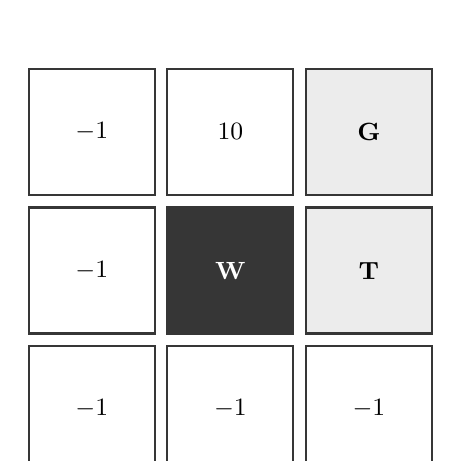
\begin{tikzpicture}[
    scale=1.1,
    cell/.style={minimum size=1.6cm, draw=USC_Black90, line width=0.8pt, font=\small\bfseries, anchor=center}
]
\node[cell] at (0, 3.2) {$-1$};
\node[cell] at (1.6, 3.2) {$10$};
\node[cell, fill=USC_Black10] at (3.2, 3.2) {G};
\node[cell] at (0, 1.6) {$-1$};
\node[cell, fill=USC_Black90, text=white] at (1.6, 1.6) {W};
\node[cell, fill=USC_Black10] at (3.2, 1.6) {T};
\node[cell] at (0, 0) {$-1$};
\node[cell] at (1.6, 0) {$-1$};
\node[cell] at (3.2, 0) {$-1$};
\end{tikzpicture}
\end{center}

\textbf{After Iteration 2:}
\begin{center}
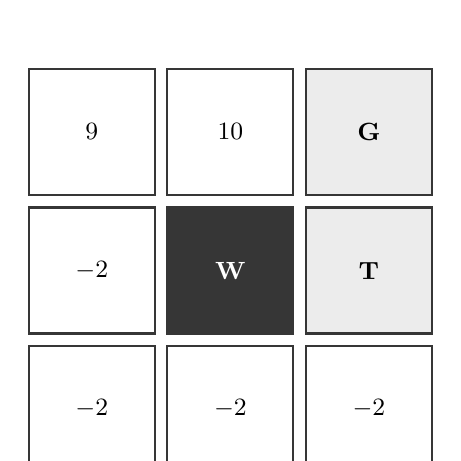
\begin{tikzpicture}[
    scale=1.1,
    cell/.style={minimum size=1.6cm, draw=USC_Black90, line width=0.8pt, font=\small\bfseries, anchor=center}
]
\node[cell] at (0, 3.2) {$9$};
\node[cell] at (1.6, 3.2) {$10$};
\node[cell, fill=USC_Black10] at (3.2, 3.2) {G};
\node[cell] at (0, 1.6) {$-2$};
\node[cell, fill=USC_Black90, text=white] at (1.6, 1.6) {W};
\node[cell, fill=USC_Black10] at (3.2, 1.6) {T};
\node[cell] at (0, 0) {$-2$};
\node[cell] at (1.6, 0) {$-2$};
\node[cell] at (3.2, 0) {$-2$};
\end{tikzpicture}
\end{center}

\item On the grid below, draw the optimal policy (one arrow per non-terminal cell indicating the best action).

\begin{stepbox}[Solution 4(c)]
The optimal path avoids the Trap and routes through the left column up to $(0,2)$, then right along the top row to Goal. The optimal policy is:
\end{stepbox}

\begin{center}
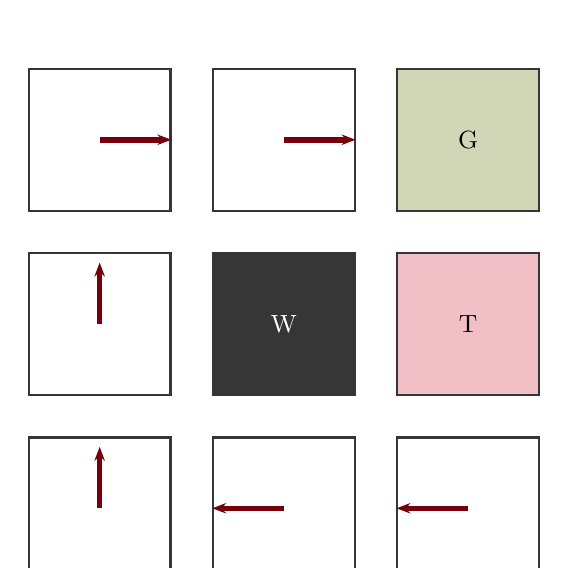
\begin{tikzpicture}[
    scale=1.3,
    cell/.style={minimum size=1.8cm, draw=USC_Black90, line width=0.8pt, font=\small, anchor=center}
]
\node[cell] (c02) at (0, 3.6) {};
\node[cell] (c12) at (1.8, 3.6) {};
\node[cell, fill=USC_Horseshoe!30] at (3.6, 3.6) {G};
\node[cell] (c01) at (0, 1.8) {};
\node[cell, fill=USC_Black90, text=white] at (1.8, 1.8) {W};
\node[cell, fill=USC_Rose!30] at (3.6, 1.8) {T};
\node[cell] (c00) at (0, 0) {};
\node[cell] (c10) at (1.8, 0) {};
\node[cell] (c20) at (3.6, 0) {};

% Policy arrows
\draw[-{Stealth[length=5pt]}, line width=2pt, USC_Garnet] (0, 0) -- (0, 0.6);        % (0,0): Up
\draw[-{Stealth[length=5pt]}, line width=2pt, USC_Garnet] (1.8, 0) -- (1.1, 0);      % (1,0): Left
\draw[-{Stealth[length=5pt]}, line width=2pt, USC_Garnet] (3.6, 0) -- (2.9, 0);      % (2,0): Left
\draw[-{Stealth[length=5pt]}, line width=2pt, USC_Garnet] (0, 1.8) -- (0, 2.4);      % (0,1): Up
\draw[-{Stealth[length=5pt]}, line width=2pt, USC_Garnet] (0, 3.6) -- (0.7, 3.6);    % (0,2): Right
\draw[-{Stealth[length=5pt]}, line width=2pt, USC_Garnet] (1.8, 3.6) -- (2.5, 3.6);  % (1,2): Right
\end{tikzpicture}
\end{center}

\end{enumerate}

% ============================================================================
% PROBLEM 5: Q-Learning Episode Trace
% ============================================================================

\question{Problem 5: Q-Learning Episode Trace}\label{prob:qlearn}

Consider the following 2-state MDP with states $\{A, B\}$ and terminal state $B_T$. Each state has two actions: $L$ and $R$.

\begin{center}
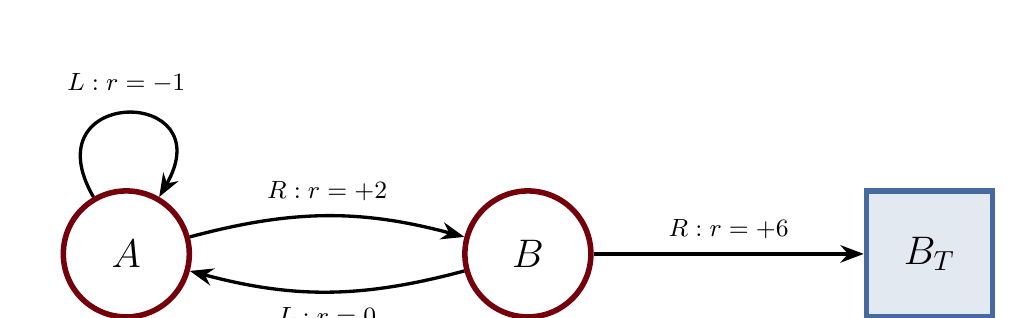
\begin{tikzpicture}[
    >=Stealth,
    scale=0.85,
    every state/.style={
        fill=white,
        draw=USC_Garnet,
        line width=2pt,
        text=black,
        minimum size=1.6cm,
        font=\bfseries\Large
    },
    every edge/.style={draw=black, line width=1.2pt, ->, >=Stealth},
    prob/.style={font=\small\bfseries, fill=white, inner sep=2pt},
    term/.style={
        fill=USC_Atlantic!15,
        draw=USC_Atlantic,
        line width=2pt,
        text=black,
        minimum size=1.6cm,
        font=\bfseries\Large
    }
]

\node[state] (A) at (0, 0) {$A$};
\node[state] (B) at (6, 0) {$B$};
\node[term] (BT) at (12, 0) {$B_T$};

\path (A) edge[loop above, looseness=5, out=120, in=60] node[prob, above=5pt] {$L: r=-1$} (A);
\path (A) edge[bend left=15] node[prob, above=3pt] {$R: r=+2$} (B);

\path (B) edge[bend left=15] node[prob, below=3pt] {$L: r=0$} (A);
\path (B) edge node[prob, above=3pt] {$R: r=+6$} (BT);

\end{tikzpicture}
\end{center}

All transitions are deterministic. Use \textbf{Q-learning} with $\alpha = 0.2$, $\gamma = 1$, and $\varepsilon = 0$ (pure greedy; break ties alphabetically by action name, i.e., $L$ before $R$).

Initialize all Q-values to zero: $Q(A,L) = Q(A,R) = Q(B,L) = Q(B,R) = 0$.

The three episode trajectories are given (not chosen by your policy---just apply the updates):

\textbf{Episode 1:} $A \xrightarrow{R} B \xrightarrow{R} B_T$

\textbf{Episode 2:} $A \xrightarrow{R} B \xrightarrow{R} B_T$

\textbf{Episode 3:} $A \xrightarrow{L} A \xrightarrow{R} B \xrightarrow{R} B_T$

\begin{enumerate}[label=(\alph*)]
\item For each step of each episode, compute the Q-learning update. Fill in the table.

\textit{Recall:} $Q(s,a) \leftarrow Q(s,a) + \alpha\big[r + \gamma \max_{a'} Q(s',a') - Q(s,a)\big]$

\begin{stepbox}[Solution 5(a)]
\textbf{Episode 1, Step 1:} $s=A, a=R, s'=B, r=+2$
\[
Q(A,R) \leftarrow 0 + 0.2[2 + 1 \cdot \max(0,0) - 0] = 0.2(2) = 0.40
\]

\textbf{Episode 1, Step 2:} $s=B, a=R, s'=B_T, r=+6$
\[
Q(B,R) \leftarrow 0 + 0.2[6 + 0 - 0] = 1.20
\]

\textbf{Episode 2, Step 1:} $s=A, a=R, s'=B, r=+2$. Now $\max_{a'}Q(B,a') = 1.20$.
\[
Q(A,R) \leftarrow 0.40 + 0.2[2 + 1.20 - 0.40] = 0.40 + 0.2(2.80) = 0.96
\]

\textbf{Episode 2, Step 2:} $s=B, a=R, s'=B_T, r=+6$
\[
Q(B,R) \leftarrow 1.20 + 0.2[6 + 0 - 1.20] = 1.20 + 0.2(4.80) = 2.16
\]

\textbf{Episode 3, Step 1:} $s=A, a=L, s'=A, r=-1$. $\max_{a'}Q(A,a') = 0.96$.
\[
Q(A,L) \leftarrow 0 + 0.2[-1 + 0.96 - 0] = 0.2(-0.04) = -0.008
\]

\textbf{Episode 3, Step 2:} $s=A, a=R, s'=B, r=+2$. $\max_{a'}Q(B,a') = 2.16$.
\[
Q(A,R) \leftarrow 0.96 + 0.2[2 + 2.16 - 0.96] = 0.96 + 0.2(3.20) = 1.60
\]

\textbf{Episode 3, Step 3:} $s=B, a=R, s'=B_T, r=+6$
\[
Q(B,R) \leftarrow 2.16 + 0.2[6 + 0 - 2.16] = 2.16 + 0.2(3.84) = 2.928
\]
\end{stepbox}

\begin{resultsbox}
\begin{center}
\begin{tabular}{ccccccl}
\toprule
\textbf{Ep.} & \textbf{Step} & $\mathbf{s}$ & $\mathbf{a}$ & $\mathbf{s'}$ & $\mathbf{r}$ & \textbf{New $Q(s,a)$} \\
\midrule
1 & 1 & $A$ & $R$ & $B$ & $+2$ & $Q(A,R) = 0.400$ \\[0.4em]
1 & 2 & $B$ & $R$ & $B_T$ & $+6$ & $Q(B,R) = 1.200$ \\[0.4em]
\midrule
2 & 1 & $A$ & $R$ & $B$ & $+2$ & $Q(A,R) = 0.960$ \\[0.4em]
2 & 2 & $B$ & $R$ & $B_T$ & $+6$ & $Q(B,R) = 2.160$ \\[0.4em]
\midrule
3 & 1 & $A$ & $L$ & $A$ & $-1$ & $Q(A,L) = -0.008$ \\[0.4em]
3 & 2 & $A$ & $R$ & $B$ & $+2$ & $Q(A,R) = 1.600$ \\[0.4em]
3 & 3 & $B$ & $R$ & $B_T$ & $+6$ & $Q(B,R) = 2.928$ \\[0.4em]
\bottomrule
\end{tabular}
\end{center}
\end{resultsbox}

\item State all four Q-values after the 3 episodes are complete.

\begin{resultsbox}
\[
\boxed{Q(A,L) = -0.008, \quad Q(A,R) = 1.600, \quad Q(B,L) = 0.000, \quad Q(B,R) = 2.928}
\]
\end{resultsbox}

\item What is the greedy policy $\pi(s) = \arg\max_a Q(s,a)$ for each state?

\begin{resultsbox}
\[
\boxed{\pi(A) = R \quad (\text{since } 1.600 > -0.008)}, \qquad \boxed{\pi(B) = R \quad (\text{since } 2.928 > 0)}
\]
\end{resultsbox}

\end{enumerate}

% ============================================================================
% PROBLEM 6: Exploration vs Exploitation
% ============================================================================

\question{Problem 6: Exploration vs.\ Exploitation}\label{prob:explore}

\begin{enumerate}[label=(\alph*)]
\item Suppose an agent is in a state with three available actions $\{a_1, a_2, a_3\}$ and current Q-values:
\[
Q(s, a_1) = 5.0, \qquad Q(s, a_2) = 3.2, \qquad Q(s, a_3) = 7.1
\]
Under an $\varepsilon$-greedy policy with $\varepsilon = 0.4$, compute the probability of selecting each action.

\begin{stepbox}[Solution 6(a)]
Under $\varepsilon$-greedy with $|\mathcal{A}| = 3$ actions:
\begin{itemize}[nosep]
\item The greedy action is $a_3$ (highest Q-value of 7.1).
\item Each action gets a base probability of $\varepsilon / |\mathcal{A}| = 0.4/3 = 2/15$ from random exploration.
\item The greedy action gets an additional $1 - \varepsilon = 0.6$ probability.
\end{itemize}
\end{stepbox}
\begin{resultsbox}
\[
\boxed{P(a_1) = \frac{2}{15} \approx 0.133}, \qquad
\boxed{P(a_2) = \frac{2}{15} \approx 0.133}, \qquad
\boxed{P(a_3) = 0.6 + \frac{2}{15} = \frac{11}{15} \approx 0.733}
\]
Verification: $\frac{2}{15} + \frac{2}{15} + \frac{11}{15} = \frac{15}{15} = 1$ \checkmark
\end{resultsbox}

\item Suppose $\varepsilon$ starts at $\varepsilon_0 = 1.0$ and decays multiplicatively each episode by a factor of $0.99$:
\[
\varepsilon_k = \varepsilon_0 \cdot 0.99^k
\]
After how many episodes $k$ is $\varepsilon_k < 0.05$? Solve exactly using logarithms.

\begin{stepbox}[Solution 6(b)]
\begin{align*}
0.99^k &< 0.05 \\
k \ln(0.99) &< \ln(0.05) \\
k &> \frac{\ln(0.05)}{\ln(0.99)} \qquad \text{(inequality flips since } \ln(0.99) < 0\text{)} \\
k &> \frac{-2.9957}{-0.01005} = 298.07
\end{align*}
\end{stepbox}
\begin{resultsbox}
\[
\boxed{k = 299}
\]
is the first episode where $\varepsilon_k < 0.05$. ($\varepsilon_{299} = 0.99^{299} \approx 0.0495 < 0.05$; $\varepsilon_{298} \approx 0.0500 \geq 0.05$.)
\end{resultsbox}

\item In 3--5 sentences, explain: Why is exploration important in the early stages of learning? Why is it beneficial to decay $\varepsilon$ over time rather than keeping it fixed?

\begin{stepbox}[Solution 6(c)]
In the early stages of learning, the agent's Q-value estimates are inaccurate (typically initialized to zero or random values), so the greedy action with respect to current estimates is unlikely to be truly optimal. Exploration allows the agent to visit state--action pairs it has not yet tried, gathering information that improves Q-value estimates across the entire state--action space. Without sufficient exploration, the agent may converge to a suboptimal policy because it never discovers higher-reward paths.

Decaying $\varepsilon$ over time is beneficial because it allows the agent to transition from an \emph{information-gathering} phase to an \emph{exploitation} phase. As training progresses and Q-values become more accurate, continued random exploration wastes reward by choosing known-suboptimal actions. A decaying schedule balances the exploration--exploitation tradeoff: explore broadly when uncertain, then increasingly commit to the learned policy as confidence grows.
\end{stepbox}

\end{enumerate}

% ============================================================================
% END OF DOCUMENT
% ============================================================================

\end{document}
